\documentclass[]{beamer}

\usetheme[displaysinglefooter,displaytocsection]{ISG}


\title{Example Beamer Presentation}
\subtitle{A Demonstration of the ISG Beamer Template}  
\author[R. Lee \& D. Hutchinson]{Robert Lee and Daniel Hutchinson}
\institute{Information Security Group,\\
Royal Holloway}

\begin{document}
\begin{frame}
	\titlepage
\end{frame}

\begin{frame}\frametitle{Presentation Contents}
	\tableofcontents
\end{frame}

\section{Available Headers}
\begin{frame}\frametitle{Different Headers Provided by ISG beamer theme}
\begin{itemize}
	\item There are three headers provided by the ISG beamer theme: \texttt{blurredheader}, \texttt{sharpheader} and \texttt{splitheader}.
	\item \texttt{sharpheader} is the default and is used on this presentation. It uses the \texttt{miniframes} outer theme.
	\item \texttt{blurredheader} is similar to \texttt{sharpheader}, however there is a colour blur between the boxes in the header.  It uses the \texttt{smoothbars} outer theme.
	\item \texttt{splitheader} uses the header from the \texttt{shadow} outer theme with a modification which limits the number of sections displayed in the header to three.
	\item Examples of each header can be found in the following slides.
\end{itemize}
\end{frame}

\begin{frame}\frametitle{\texttt{sharpheader}}
\begin{center}
	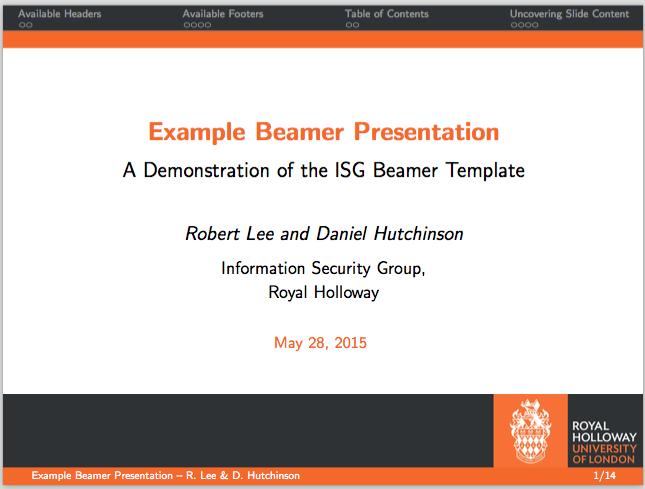
\includegraphics[scale=0.4]{graphics/sharpheader.png}
\end{center}
\end{frame}

\begin{frame}\frametitle{\texttt{blurredheader}}
\begin{center}
	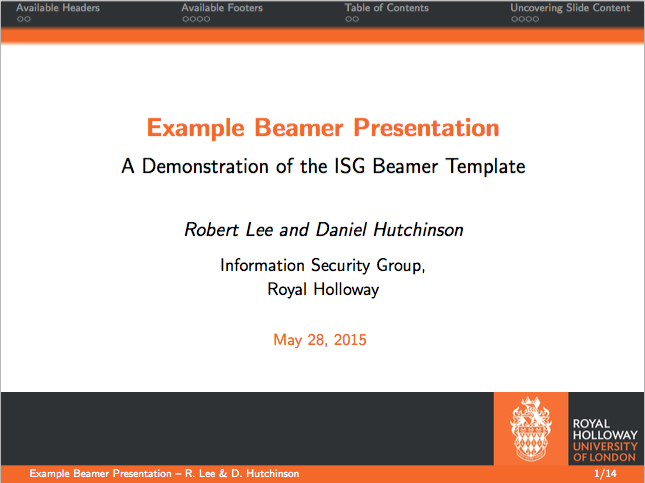
\includegraphics[scale=0.4]{graphics/blurredheader.png}
\end{center}
\end{frame}

\begin{frame}\frametitle{\texttt{splitheader}}
\begin{center}
	
\includegraphics[scale=0.4]{graphics/splitheader.png}
\end{center}
\end{frame}

\section{Available Footers}
\begin{frame}\frametitle{Split or Single?}
\begin{itemize}
	\item Two different footers are provided by the ISG style.  They are called split and single
	\item The single footer is the default and sets the footer as one solid orange bar
	\item The split footer divides the footer into two halves, orange and grey.  The title and authors are displayed on different sides of the orange/grey split.
	\item The footers are chosen by passing parameters when using the ISG theme, e.g.\ by \texttt{\textbackslash usetheme[displaysinglefooter]\{ISG\}} or \texttt{\textbackslash usetheme[displaysplitfooter]\{ISG\}}.
	\item Examples of each footer can be found in the following slides.
\end{itemize}
\end{frame}

\begin{frame}\frametitle{\texttt{singlefooter}}
\begin{center}
	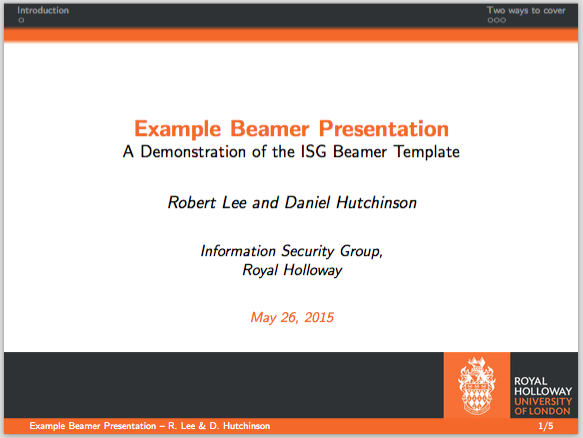
\includegraphics[scale=0.4]{graphics/singlefooter.png}
\end{center}
\end{frame}

\begin{frame}\frametitle{\texttt{splitfooter}}
\begin{center}
	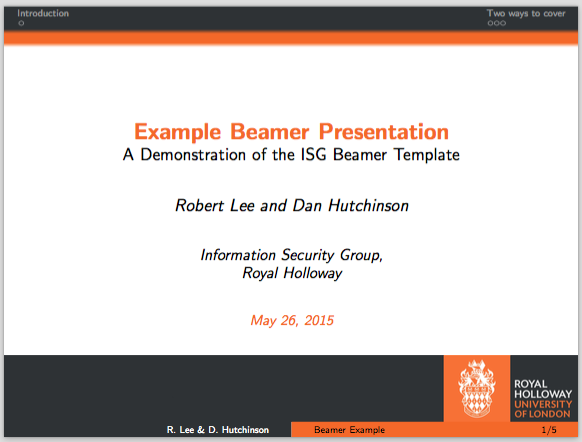
\includegraphics[scale=0.4]{graphics/splitfooter.png}
\end{center}
\end{frame}

\section{Table of Contents}
\begin{frame}\frametitle{Showing progress through the presentation}
\begin{itemize}
	\item The beamer style is also able to show a table of contents whenever a new section or subsection is begun.
	\item These options are selected by passing the appropriate parameters when using the ISG theme.
	\item E.g.\ \texttt{\textbackslash usetheme[displaytocsection]\{ISG\}} or \texttt{\textbackslash usetheme[displaytocsubsection]\{ISG\}}.
	\item These can be used together with other options in the ISG style, e.g.\ this presentation uses the following\\ {\scriptsize\texttt{\textbackslash usetheme[displaysinglefooter, displaytocsection]\{ISG\}}}
\end{itemize}
\end{frame}

\setbeamercovered{invisible}
\section{Uncovering Slide Content}
\begin{frame}\frametitle{Invisible Covering}
\begin{itemize}
	\item I'm the first item!
	\pause
	\item I was invisible!
	\pause
	\item Invisible is selected by \texttt{\\setbeamercovered\{invisible\}}
\end{itemize}
\end{frame}

\setbeamercovered{transparent}
\begin{frame}\frametitle{Transparent covering}
\begin{itemize}
	\item I'm the first item!
	\pause
	\item I was transparent!
	\pause
	\item Transparent is selected by \texttt{\\setbeamercovered\{transparent\}}
\end{itemize}
\end{frame}

\section{One more thing}
\begin{frame}\frametitle{A quirk of the ISG style}
\begin{itemize}
	\item The title page has a few quirks due to the way it has been implemented.
	\item This means that you have to build your .tex file three times before things are in the right place.
	\item This is less tedious if you use a make file!
\end{itemize}
\end{frame}

\end{document}


